\documentclass{article}
\usepackage{graphicx}
\usepackage{hyperref}

\begin{document}
\author{James Lacroix (V00897338)}
\title{Retrieving and analysing the average clock drift rate for a non-time synchronized machine}

\maketitle

\section*{Summary}
I wrote a simple SNTP client in go to calculate the average drift rate for a machine and the analysed the results with python. \\
\\
The test machine was a raspberry pi 3b, on wifi, with an inadequate power supply. The NTP client was disabled during the tests. \\
\\
The code used to retrieve these results can be found here: \\
\url{https://github.com/LacroixJ/sntp-go}



\section*{Average RTT}
The average return trip time was 94.51ms, a fairly long time. Other devices on the same network could get an RTT of about 60ms to the same server. This can probably be attributed to the combination of wifi and a poor power supply causing throttling. 



\section*{Average Clock Drift Rate}
Calculating the average clock drift rate was done by taking the difference between a clock drift, and the clock drift of the previous iteration (for each iteration), making a list of these values, and then taking the average of the entire list. Finally I divided the total result by 10 because I took one measurement every 10 seconds. 

\subsection*{Results}
The average clock drift rate was found to be 2.28 microseconds per second. That is, for every second, the raspberry pis clock would increase by 1 second + 2.28 microseconds.\\
\\
By the end of the 12 hour test, the internal clock had drifted roughly 20ms in total from its starting state. 
This number seems to be very low, but it makes sense when thinking about what kind of machine the test was being run on.\\ 
\\
The raspberry pi is often used for embedded systems and small projects where it won't have access to an NTP server. To account for this, the hardware most likely has a better internal clock than most other motherboards would. 



\section*{Packet Loss}
The failure rate, or the packet loss rate was 0.14\% with a time-out of 1 second. Normally the time-out for an application to receive a transmission back from an NTP server would be much longer, on the order of 30 seconds to a minute. However in this case I was a bit harsher because I have very good internet, and uptime is essential for ntp servers, meaning that I may have not seen a single packet drop during my 12 hour test with a longer time-out. \\
\\
This does mean that any hiccups in the network that caused the RTT to go over 1 second would show as a 'lost packet'. I was more concerned with getting a measurement at all over such a short interval. 1 second is over 10 times the average rtt so it would be unlikely to see many of these false positives. \\
\\
Any packet that was considered timed out was ignored if received later. 


\section*{Histogram of average drift}

A histogram of average packet drift rates was generated using Python and the matplotlib library. Results with over 15 microseconds of drift were ignored because they skewed the results too much. \\
\\
These results are interesting, because almost no values were under 2 microseconds but there were many above it. One thing that the histogram does not show is that the results got closer and closer to 2 microseconds as the tests progressed.\\
\\
This could be because of the load on the machine was varying at the start, because I was still doing other things on it, making the values higher. \\
\\
It is clear that with no load the pi will have around 2 microseconds of drift per second, but it can vary greatly depending on what is happening with the system. \\
\\
For a time critical application, this could have disastrous consequences, so it should be accounted that the drift can vary a decent amount especially during short time periods.\\
 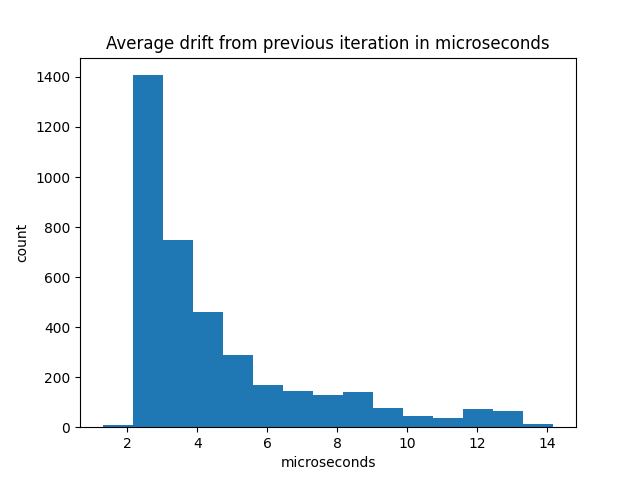
\includegraphics[scale=0.8]{../average_drift_histo.png}                                              
 
  
  
  \end{document}
